\section{Part 5.1 Assignment of the boat parameters}
\subsection{a}
Given the equations from \todo{Cite lab text}
\begin{subequations}
\begin{align}
    \dot{\xi} &= \psi_\omega\\
    \dot{\psi}_\omega &= -\omega^2_0 \xi_\omega - 2 \lambda \omega_0 \psi_\omega + K_\omega \omega_\omega\\
    \dot{\psi} &= r\\ \label{eq:start_psi}
    \dot{r} &= -\frac{1}{T} r + \frac{K}{T} (\delta-b)\\ \label{eq:start_r}
    \dot{b} &= \omega_b\\
    y &= \psi + \psi_\omega + v
\end{align}
\end{subequations}
We want to find the transfer function, $H(s)$, from $\delta$ to $\psi$. Taking the Laplace transform of \cref{eq:start_r} we get 
\begin{align*}
    \mathcal{L}\{\dot{r}\}(s) &= \mathcal{L}\{{-\frac{1}{T} r + \frac{K}{T}
    (\delta - b)}\}(s)\\
    s r&=-\frac{1}{T} r + \frac{K}{T}(\delta - b)\\
    r &= \frac{K}{T}(\delta-b) \frac{1}{s+\frac{1}{T}}
\end{align*}
Assuming there is no disturbances and substituting into  \cref{eq:start_psi} we then get
\begin{align}
    H(s) &= \frac{K}{s(Ts+1)}
\end{align}
\subsection{b}
Use the plots and show the derivation of the parameters K and T. Measured amplitude from scopes
$K = 0.1559$ and $T = 71.6865$
\begin{align*}
    \omega_1 &= 0.005\\
    \omega_2 &= 0.05\\
    K &= A_1\omega_1\sqrt{T^2\omega_1^2+1}\\
    T &= \sqrt{\frac{A_2^2\omega_2^2-A_1^2\omega_1^2}{A_1^2\omega_1^4-A_2^2\omega_2^4}}
\end{align*}
$$K = A_1\omega_1\sqrt{T^2\omega_1^2+1}$$

$$T = \sqrt{\frac{A_2^2\omega_2^2-A_1^2\omega_1^2}{A_1^2\omega_1^4-A_2^2\omega_2^4}}$$

\subsection{c}
Setting the measurement cursors at the peak without noise. 
Repeating the procedure we get $K = 0.3572$ and $T = 444.6904$
Is it possible to get good estimates?\\
We get decent estimates but is not that good when setting the frequency to 0.05. Maybe because the frequency of the waves is close to the frequency of the sine. 
\subsection{d}
Applied a step on both the full system model in Simulink and also on the transfer function using MATLAB. 
\begin{figure}
    \centering
    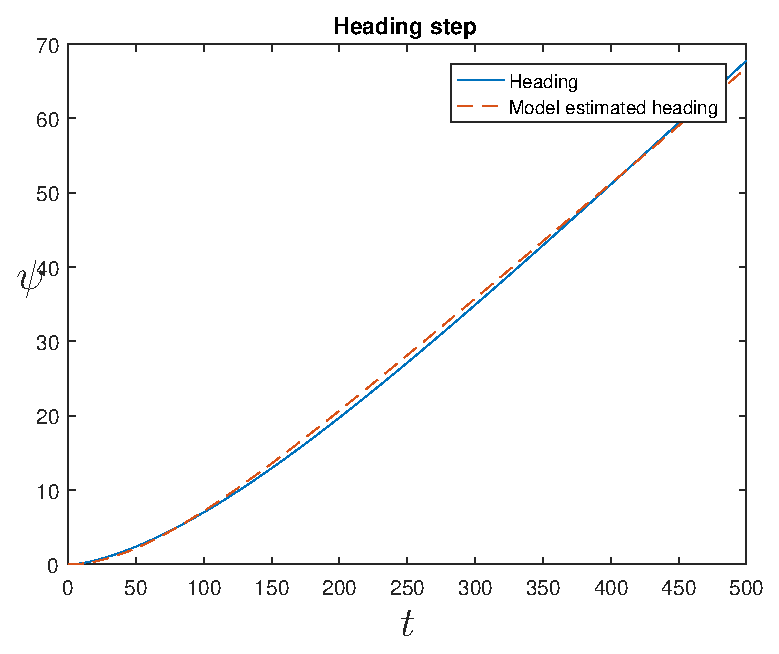
\includegraphics{figures/plots/p5p1d.eps}
    \caption{Caption\todo{}}
    \label{fig:my_label}
\end{figure}